\documentclass[pss]{wiley2sp} % provides pss two-column style
\usepackage{amsmath}
\usepackage{subfig}

\renewcommand{\arraystretch}{1.2} % please do not remove or change
\tolerance=400
\emergencystretch=10pt

\begin{document}

% Title of the article
\title{Nonlinear optical responses in hydrogenated graphene structures}

% Authors
\author{
    Reinaldo Zapata-Pe\~na\textsuperscript{\Ast,\textsf{\bfseries 1}},
    Sean M. Anderson\textsuperscript{\Ast,\textsf{\bfseries 1}},
    Bernardo S. Mendoza\textsuperscript{\Ast,\textsf{\bfseries 1}},
    Anatoli I. Shkrebtii\textsuperscript{\textsf{\bfseries 2}}}

% Abbreviated list of authors for the page headers
\titlerunning{Optical spin injection, current injection, and SHG study of
hydrogenated graphene}
\authorrunning{R. Zapata-Pe\~na et al.}

%E-mail-address of corresponding author
\mail{e-mail
  \textsf{bms@cio.mx}, Phone:
  +52-477-441-4200, Fax: +52-477-441-4209}

% author's affiliations/addresses
\institute{%
  \textsuperscript{1}\,Centro de Investigaciones en \'Optica, Le\'on,
  Guanajuato 37150, M\'exico\\
  \textsuperscript{2}\,University of Ontario, Institute of Technology, Oshawa,
  ON, L1H 7L7, Canada}

\received{XXXX, revised XXXX, accepted XXXX}
\published{XXXX} % do not change, will be filled in by the publisher

% Please select about four verbal keywords for your manuscript.
\keywords{graphene, spin polarization, current injection, second-harmonic.}

\abstract{%
\abstcol{%
We present a theoretical study of spin and current injection, and 
second-harmonic generation via optical means from the C$_{16}$H$_{8}$-alt and
C$_{16}$H$_{8}$-up graphene structures. The incidence of circularly polarized
light onto nonmagnetic semiconductors produces spin-polarized electrons in the
conduction bands. Current injection and second-harmonic generation are
nonlinear, second-order effects that can be produced from both the bulk and
surface of noncentrosymmetric materials. In centrosymmetric materials, these
effects can only be observed at the surface where the inversion symmetry is
broken.} {We also report results for the degree of spin polarization, current
injection, and second-harmonic generation calculated within a full electronic
band structure scheme at the DFT-LDA level using a planewave basis. Our
results show that these effects can be optically generated in both the
C$_{16}$H$_{8}$-alt and C$_{16}$H$_{8}$-up structures, presenting an
anisotropic behavior. We obtain a maximum degree of spin polarization of 39\%
for C$_{16}$H$_{8}$-alt, and 57\% for C$_{16}$H$_{8}$-up, which are
promising results for potential applications in spintronics.}}


\maketitle


\section{Introduction}\label{sec:intro}

Graphene is an allotrope of carbon with a planar, hexagonal, two-dimensional honeycomb structure with one carbon atom at each vertex, see Fig. \ref{fig:structures}. The first samples were produced by exfoliating graphite into carbon sheets, eventually producing a monolayer of carbon atoms. Graphene production has been substantially improved since then using other methods, such as chemical vapor deposition, that provides better control over the final structure. Graphene has attracted great interest due to its distinctive properties, such as the fractional quantum Hall effect at room temperature, and excellent thermal transport properties \cite{geimNM07,geimNM07,reinaNL08,bottegoniAPL13,balandinNL08}. Graphene has metallic behavior but has a variable band gap that can be tuned by changing the surface area \cite{hanPRL07}, applying an electric field \cite{zhangN09}, applying uniaxial strain \cite{niACSN08}, or by doping. Previous works have explored doping with boron, nitrogen \cite{guoIJ11}, and hydrogen \cite{eliasS09,guisingerNL09,samarakoonACSN10}.

When graphene is hydrogenated it is possible to obtain different spatial configurations through varying the amount and location of the hydrogen bonds. In this paper we present a study of two 50\% hydrogenated graphene structures, C$_{16}$H$_{8}$-alt and C$_{16}$H$_{8}$-up, both presenting a discernible band gap. As shown in Fig. \ref{fig:altstrc} and \ref{fig:upstrc}, when a hydrogen atom is bonded to a carbon atom on the graphene plane, it pulls the carbon atom from the plane modifying the carbon-carbon bond length, and then opening the band gap \cite{samarakoonACSN10}. The \emph{alt} case (Fig. \ref{fig:altstrc}) has hydrogen on both sides of the sheet, alternating between the upper and lower faces of the plane. The \emph{up} case (Fig. \ref{fig:upstrc}) has all the hydrogens on a single side, producing a zig-zag form in the carbon lattice. In this paper we conduct a theoretical study of three optical nonlinear phenomena in the structures mentioned above: the degree of spin polarization (DSP), $\mathcal{D}(\omega)$, optical current injection, $\mathbf{\dot{J}}(\omega)$, and second-harmonic generation (SHG). We describe these as follows.


\begin{figure}[t]
\subfloat[Top and side view of pristine graphene structure.]
{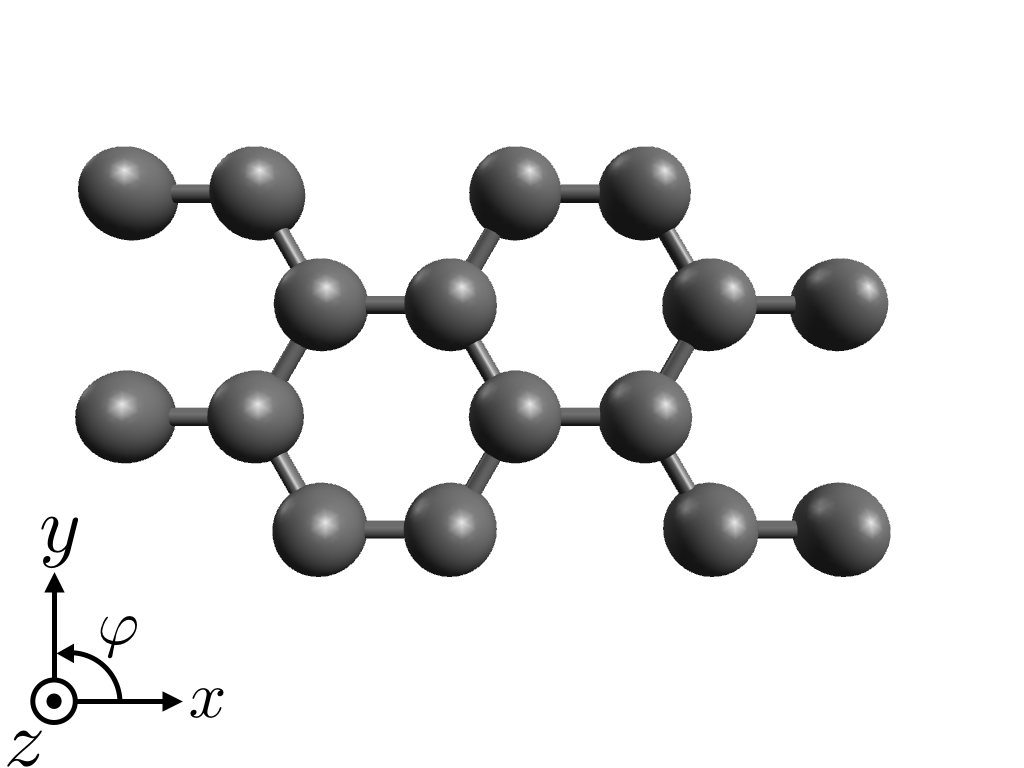
\includegraphics[width=0.49\linewidth]{figures/graph1}
 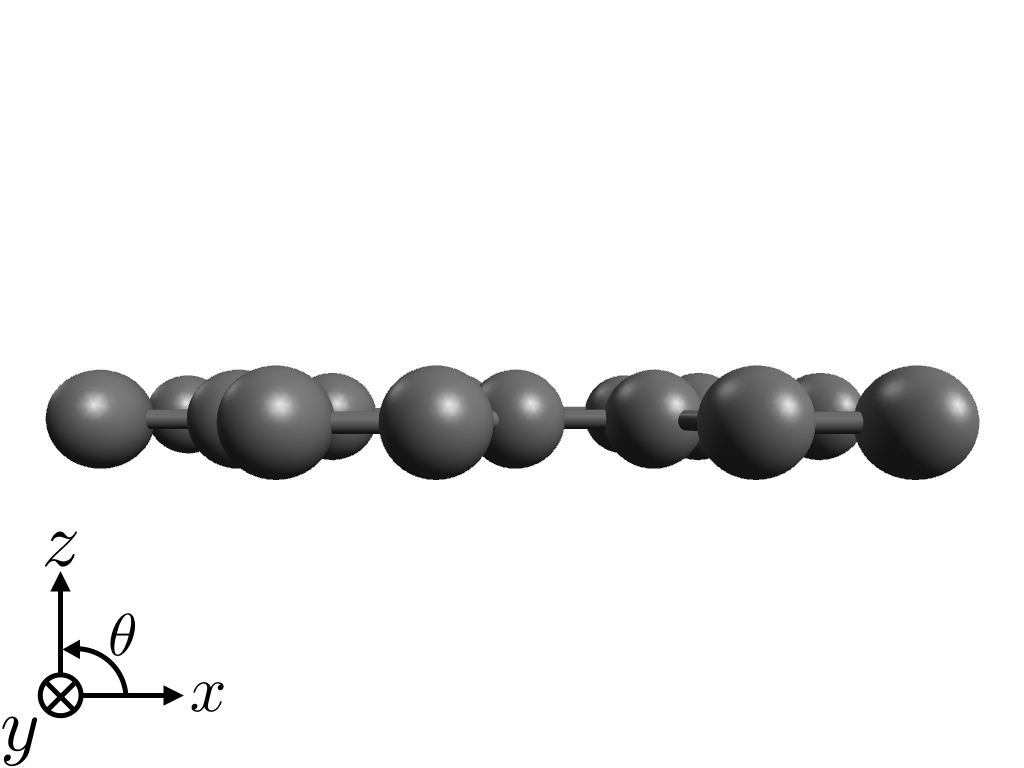
\includegraphics[width=0.49\linewidth]{figures/graph2}\label{fig:graphenestrc}}
\\
\subfloat[Top and side view of C$_{16}$H$_{8}$-alt graphene structure.]
{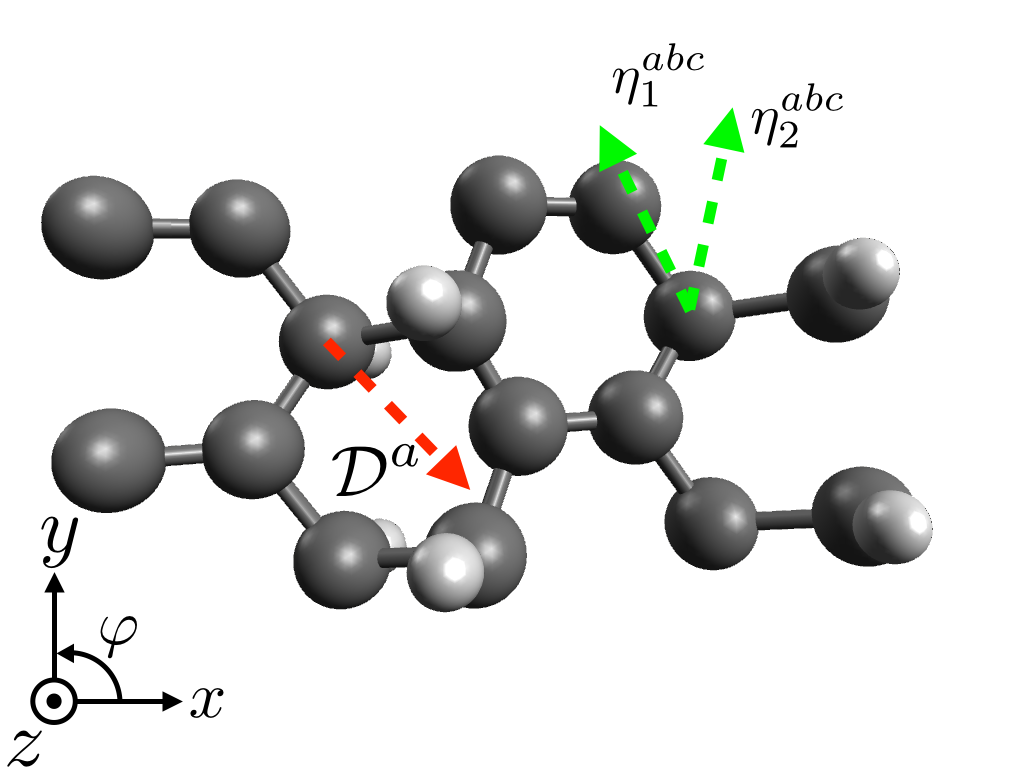
\includegraphics[width=0.49\linewidth]{figures/alt1}
 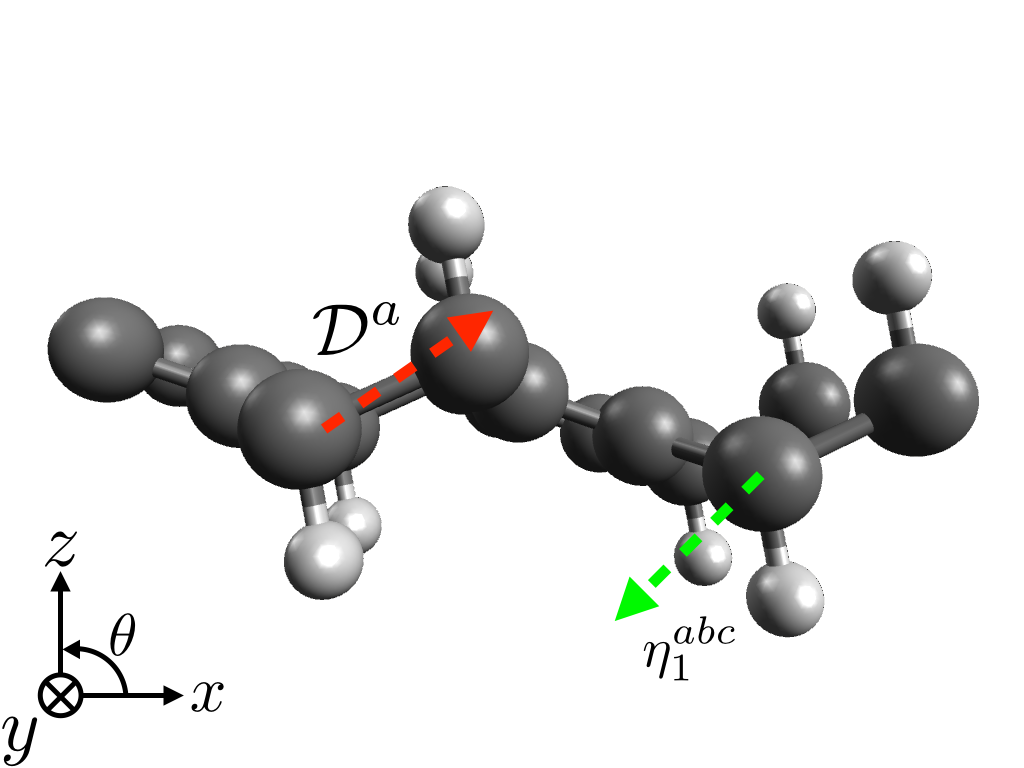
\includegraphics[width=0.49\linewidth]{figures/alt2}\label{fig:altstrc}}
\\
\subfloat[Top and side view of C$_{16}$H$_{8}$-up graphene structure.]
{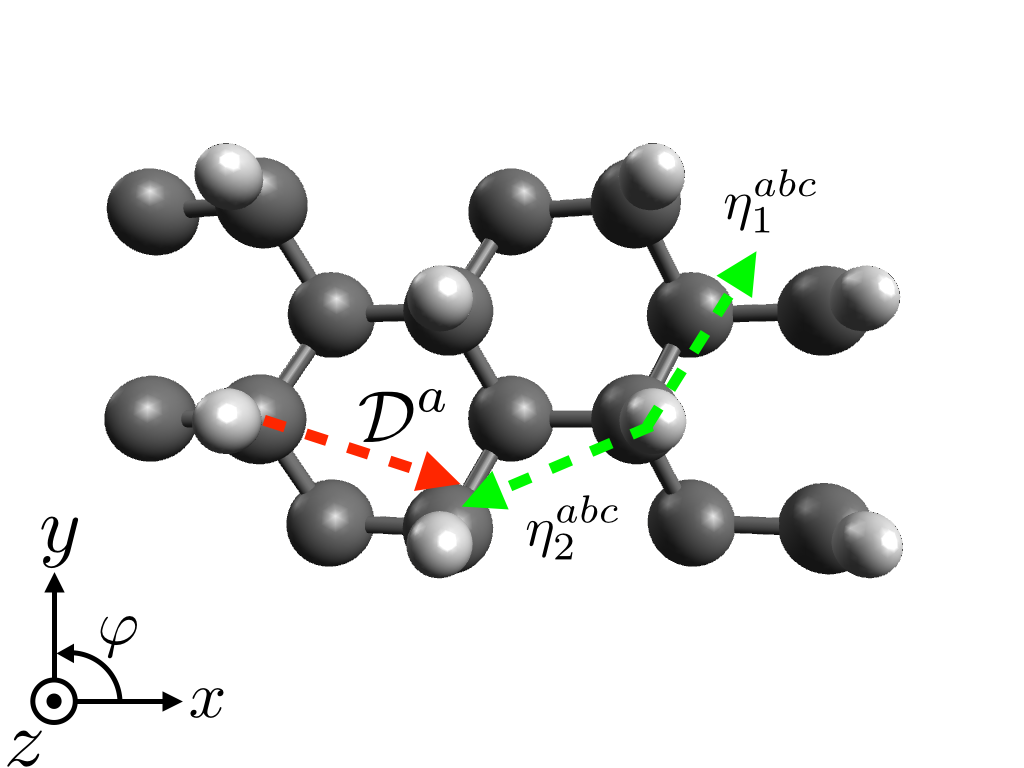
\includegraphics[width=0.49\linewidth]{figures/up1}
 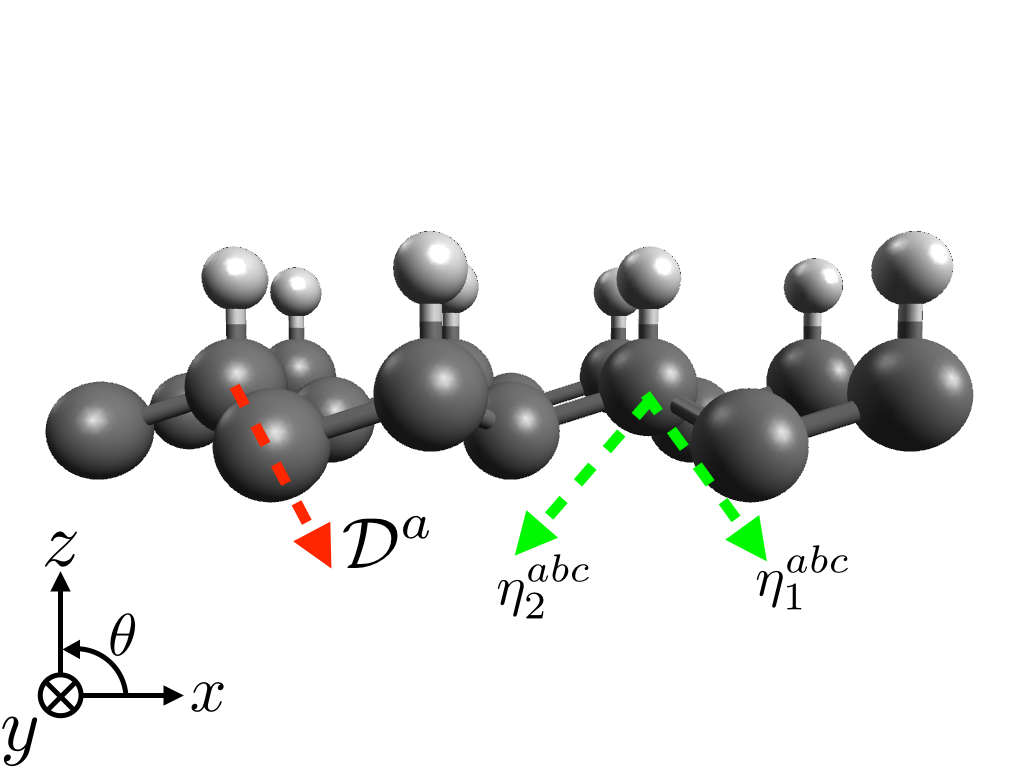
\includegraphics[width=0.49\linewidth]{figures/up2}\label{fig:upstrc}}
\caption{(Color online) Diagrams of the graphene (\ref{fig:graphenestrc}), \emph{alt} (\ref{fig:altstrc}), and \emph{up} (\ref{fig:upstrc}) structures. The light (dark) spheres correspond to hydrogen (carbon) atoms. For each sibfigure the left side corresponds to a point of view in the $xy$ plane and the right to the $xz$ plane. The red (green) dashed arrows in \ref{fig:altstrc} and \ref{fig:upstrc} represent the direction where the $\mathcal{D}(\omega)$ ($\eta^{abc}(\omega)$) point in the corresponding $xy$ and $xz$ plane. This information is explained in subsections \ref{subsec:results-DSP} and \ref{subsec:results-eta}.\label{fig:structures}}
\end{figure}

\subsection{Degree of spin polarization}

The injection and detection of spin polarized electrons into nonmagnetic materials is the core of spintronics \cite{vzuticRMP04,fertRMP08} and an important  problem in condensed matter theory.
The idea of creating and detecting spin polarization from light dates to the 1960s \cite{LampelPRL68} and in Ref. \cite{dyakonovOO84} it was shown that conversion of angular momentum of light into electron spin and vice versa is very efficient in III-IV semiconductors. The optical spin injection is characterized through the dimensionless quantity of DSP, $\mathcal{D}(\omega)$, which is a function of the photon frequency, $\omega$. The DSP quantifies the fraction of injected electrons into the conduction bands that are spin polarized.
The process of optical spin injection appears when circularly polarized light is incident on a semiconducting material \cite{dyakonovOO84}. This allows electrons to move from the valence to the conduction bands and the resulting polarization is produced by the interaction between the electron spin and its motion caused by the spin-orbit coupling in the material. DSP can be calculated with full band structure local-density approximation (LDA) and $\textbf{k}\cdot\textbf{p}$ methods \cite{nastosPRB07,cabellosPRB09}. There are theoretical reports of DSP calculations for bulk media (Si, GaAs, CdSe, and Ge semiconductors) \cite{nastosPRB07,cabellosPRB09} and surfaces (Si(111):In, Si(111):As, GaAs(110):Sb, GaAs(110), and Si(111) with $4\times2$ and $8\times2$ reconstructions) \cite{mendozaPRB12,arzatePRB14}. 

\subsection{Optical current injection}

The control of chemical process is of interest in science and engineering. The optical current injection, $\mathbf{\dot{J}}(\omega)$ , is a surface-sensitive optical effect that offers the potential to control chemical reactions \cite{bhatPRB05,hachePRL97}. In noncentrosymmetric crystals, a photocurrent can be injected with a single optical beam coming  from the interference of one-photon absorption processes associated with different linear polarizations of the light. From the total of the 32 crystal classes only 21 are noncentrosymmetric and this process is only allowed in 18 of them. Crystals corresponding to the $\bar{6}m\bar{2}$, $\bar{6}$, and $\bar{4}$$\bar{3}$m are the exceptions \cite{sipePRB00}. The one-photon current injection is characterized by the current injection tensor, $\eta(0; \omega, − \omega)$, which is a particular case of $\eta(\omega_{1}-\omega_{2}; \omega_{1},-\omega_{2})$, from where $\omega_{1}$ and $\omega_{2}$ are frequencies of identical photons. Here we will denote its frequency dependence as $\eta(\omega)$. The optical current injection process can be understood as a quantum effect of one photon absorption events associated with different linear polarizations of light. For this phenomenon the electromagnetic field provides the energy of the promoted carriers up to the rise in momentum is provided by the crystal lattice \cite{arzatePRB14}. The process of optical current injection can be generated in bulk semiconductors \cite{hachePRL97,sipePRB00}, two-dimensional systems \cite{melePRB00,cabellosPRB11}, and one-dimensional nanotubes \cite{melePRB00}. 

\subsection{Second-harmonic generation}

The characterization of structures and interfaces is an important issue in the development of microelectronics, nanomaterials, semiconductors, and other areas of interest in science and technology. Some techniques to characterize surfaces, like emission or scattering of electrons, require ultrahigh vacuum conditions and provide no access to buried systems. Second-harmonic generation (SHG) is a nonlinear process in which pairs of photons of the same frequency are annihilated to produce new photons with twice the energy and half of the wavelength of the initial photons. SHG spectroscopy technique brings the possibility to study properties of materials and has a non invasive, nondestructive and surface sensitive nature. Using this technique it is possible to characterize properties like phase transitions, atomic structure, molecular and atomic physisorption, structure deformation, and many others \cite{dadapPRB97,godefroyAPL96,salazarPRB14,mendozaPRL98}. The process is suitable with non-ultrahigh vacuum conditions even if the system is buried under transparent overlayers. The macroscopic basis of SHG, which describe the phase, intensity, and polarization of detected fields to nonlinear and linear susceptibilities at the material interface is described in \cite{downerSIA01}. In centrosymmetric systems the bulk SHG signal is identically zero but the SHG process can occur at the surface where the inversion symmetry is broken.  

This paper is organized as follows. In Sec. \ref{sec:theory} we present the theory and formulas that describe the DSP, optical current injection, and SHG. In Sec. \ref{sec:results} we describe the details of the calculations and the corresponding spectra for the respective \emph{alt} and \emph{up} structures. Finally, we give our conclusions in Sec. \ref{sec:conclusions}.


\section{Theory}\label{sec:theory}

In this section we report a summary of the formalism that describes the three phenomena presented here. They have been already reported before with more details and it is possible to consult Refs. \cite{nastosPRB07,mendozaPRB12} for DSP, Refs. \cite{cabellosPRB11,sipePRB00} for optical current injection, and Ref. \cite{andersonPRB15} for SHG.


\subsection{Optical spin injection}\label{sec:theory-DSP}

The DSP, $\mathcal{D}^{a}(\omega)$, along a given direction $a$, is defined as
\begin{equation}\label{eq:da}
\mathcal{D}^{a}(\omega)=\frac{\dot{S}^{abc}(\omega)}{(\hbar/2)\dot{n}^{bc}(\omega)},
\end{equation}
where the spin generation rate, $\dot{S}^{abc}(\omega)$, and the carrier generation rate, $\dot{n}^{bc}(\omega)$,  are given by 
\begin{align*}
\dot{S}^{abc}(\omega) &= \zeta^{abc}(\omega)E^{b}(-\omega)E^{c}(\omega), \nonumber \\ 
\dot{n}^{bc}(\omega)  &= \xi^{bc}E^{b}(-\omega)E^{c}(\omega),
\end{align*}
from where $\zeta^{abc}(\omega)$ is the spin injection rate tensor and $\xi^{bc}(\omega)$ is the carrier generation rate tensor. The spin injection rate tensor is given by
\begin{align*}\label{eq:zeta}
\zeta^{abc}(\omega) &= \frac{i\pi e^{2}}{\hbar^{2}}\int\frac{d^{3}k}{8\pi^{3}}
\sum_{vcc'}^{\prime}\text{Im}\bigl[S^{a}_{c'c}(\textbf{k})
r^{b}_{vc'}(\textbf{k})r^{c}_{cv}(\textbf{k})\nonumber\\
&\qquad+S^{a}_{cc'}(\textbf{k})
r^{b}_{vc}(\textbf{k})r^{c}_{c'v}(\textbf{k})\bigr]
\delta(\omega_{cv}(\textbf{k})-\omega),
\end{align*}
where $S^{a}_{nm}$ and $r^{a}_{nm}$ are the spin and position matrix elements. The superscripts in the previous expressions denote the three Cartesian coordinates. The carrier generation rate tensor is related to the linear optical response tensor by 
\begin{equation*}
\xi^{bc}(\omega)=\mathrm{Im}[(2/\hbar)\chi^{bc}].
\end{equation*}
We assume an incoming circularly polarized beam at normal incidence that propogates along the $-z$ direction, $\mathbf{E}(\omega) = E_{0}(\omega)(\hat{x} - i\hat{y})/\sqrt{2}$. Then, the expression of Eq. \eqref{eq:da} can be reduced to
\begin{equation}\label{eq:D^i}
\mathcal{D}^{a}(\omega) = 
\frac{-4i\zeta^{axy}(\omega)}
    {\hbar\left[\xi^{xx}(\omega) + \xi^{yy}(\omega)\right]}.
\end{equation}
It is possible to generate current injection along all three orthogonal directions with
an incident circularly polarized beam and so the total DSP can be obtained by
\begin{equation}\label{eq:dsptotal}
\mathcal{D}(\omega) = \sqrt{ [\mathcal{D}^{x}(\omega)]^{2} + [\mathcal{D}^{y}(\omega)]^{2} +[\mathcal{D}^{z}(\omega)]^{2}}.
\end{equation}


\subsection{Optical current injection}\label{sec:theory-OCI}

The optical current injection is defined as
\begin{equation*}
\mathbf{\dot{J}}^{a}_{\text{inj}}(\omega) =
\eta^{abc}(\omega)E_{b}(\omega)E_{c}(\omega), \label{eq:eta}
\end{equation*}
where $\eta^{abc}(\omega)$ is the surface injection current tensor and is given by
\begin{align*}
\eta^{abc}(\omega) =& \frac{i\pi e^{3}}{\hbar^{2}}\int\frac{d^{3}k}{8\pi^{3}}
\nonumber \\
\times &
\sum_{vc}\mathrm{\Delta}^{a}_{cv}(\mathbf{k})\text{Im}\big[r^{b}_{cv}(\mathbf{k})
r^{c}_{cv}(\mathbf{k})\big]\delta(\omega_{cv}(\mathbf{k})-\omega).
\end{align*}
from where $r^{a}_{nm}$ is the position matrix elements and 
\begin{equation*}
\mathrm{\Delta}^{a}_{cv} = v^{a}_{cc}(\mathbf{k})-v^{a}_{vv}(\mathbf{k}),
\end{equation*}
where $v^{a}_{nn}(\mathbf{k})=p^{a}_{nn}(\mathbf{k})/m_{e}$ is the electron velocity for a given $n$ band and the superscripts denote Cartesian coordinates.

$\eta^{abc}(\omega)$ is purely imaginary and is antisymmetric with respect to the last two indices \cite{sipePRB00,nastosPRB06}. Like in optical spin injection, it is possible to generate current injection along all three directions with an incident circularly polarized beam. Analogously to Eq. \eqref{eq:dsptotal} it is possible to have the total $\eta(\omega)$ with the relation
\begin{equation}\label{eq:etatotal}
\eta(\omega) = \sqrt{ [\eta^{abc}(\omega)]^{2} + [\eta^{abc}(\omega)]^{2} +[\eta^{abc}(\omega)]^{2}}.
\end{equation}

\subsection{Second-harmonic generation}\label{sec:theory-SHG}

For SHG we followed the formalism derived in reference \cite{andersonPRB15}. This new formalism to determine the second order susceptibility tensor including in one formulation (i) the scissors correction, (ii) the contributionof the nonlocal part of the pseudopotentials, and (iii) the cut function. For our calculation we set the cut function equal to unity which recovers the complete system response.

The second order nonlinear polarization is given by 
\begin{equation*}\label{eq:pol}
\mathcal{P}(2\omega) = \chi^{abc}(-2\omega;\omega,\omega)E^{b}(\omega)E^{c}(\omega)
\end{equation*}
where $\chi^{abc}(-2\omega;\omega,\omega)$ is the nonlinear susceptibility tensor responsible for the SHG and satisfies permutation symmetry condition. Again, the superscripts in the previous expression denote the Cartesian coordinates and if repeated are to be summed over. The expressions for the imaginary part of the tensor components $\chi^{abc}(-2\omega;\omega,\omega)$ at $1\omega$ and $2\omega$ are divided into interband ($e$) and intraband ($i$)
\begin{subequations}\label{eq:chis}
\begin{align}
\mathrm{Im}[\chi^{abc}_{e,\omega}] =  
\frac{\pi |e|^3}{2\hbar^2}\int 
&
\frac{dk^3}{8\pi^3}  
\nonumber \\
\times \sum_{vc}\sum_{q\neq(v,c)}
\frac{1}{\omega^\mathrm{\Sigma}_{cv}}
&
\left[\frac{\mathrm{Im}[\mathbf{v}^{\mathrm{\Sigma},a}_{qc}\{r^{b}_ 
{cv}r^{c}_{vq}\}]} {(2\omega^\mathrm{\Sigma}_{cv}-\omega^\mathrm{\Sigma}_{cq})} \right.
\nonumber \\
& 
\left. -\frac{\mathrm{Im}[\mathbf{v}^{\mathrm{\Sigma},a}_{vq}\{r^{c}
_{qc}r^{b}_{cv}\}]} {(2\omega^\mathrm{\Sigma}_{cv}-\omega^\mathrm{\Sigma}_{qv})}
\right]\delta(\omega^\mathrm{\Sigma}_{cv}-\omega),
\end{align}

\begin{align}
\mathrm{Im}  [\chi^{abc}_{i,\omega}]= 
\frac{\pi\vert e\vert^3}{2\hbar^2}
&
\int \frac{dk^3}{8\pi^3} 
\nonumber \\
 \times \sum_{cv}\frac{1}{(\omega^\mathrm{\Sigma}_{cv})^{2}} 
&
\Bigg[
\mathrm{Re}\left[\left\{r^{b}_{cv}\left(\mathbf{v}^
{\mathrm{\Sigma},a}_{vc}\right)_{;k^{c}}\right\}\right]
\nonumber \\
&+\frac{\mathrm{Re}\left[\mathbf{v}^{\mathrm{\Sigma},a}_{vc}\left\{
r^{b}_{cv}
\mathrm{\Delta}^{c}_{cv}\right\}\right]}{\omega^\mathrm{\Sigma}_{cv}} 
\Bigg]
\delta(\omega^\mathrm{\Sigma}_{cv}-\omega),
\end{align}

\begin{align}
\mathrm{Im}[\chi^{abc}_{e,2\omega}]= -
&
\frac{\pi |e|^3}{2\hbar^2}\int \frac{dk^3}{8\pi^3}
\nonumber \\
\times \sum_{vc}\frac{4}{\omega^\mathrm{\Sigma}_{cv}}
&
\Bigg[
\sum_{v'\ne v}\frac{\mathrm{Im}[\mathbf{v}^{\mathrm{\Sigma},a}_{vc}\{r^{b}
_{cv'}r^{c}_{v'v}\}]}
{2\omega^\mathrm{\Sigma}_{cv'}-\omega^\mathrm{\Sigma}_{cv}}
\nonumber \\ 
&
- \sum_{c'\ne c}\frac{\mathrm{Im}[\mathbf{v}^{\mathrm{\Sigma},a}_{vc}\{r^
{c}_{cc'}r^{b}_{c'v}\}]}
{2\omega^\mathrm{\Sigma}_{c'v}-\omega^\mathrm{\Sigma}_{cv}}
\Bigg]
\delta(\omega^\mathrm{\Sigma}_{cv}-2\omega),
\end{align}

\begin{align}
\mathrm{Im}[\chi^{abc}_{i,2\omega}]= 
\frac{\pi \vert e\vert^{3}}{2\hbar^2}
&
\int \frac{dk^3}{8\pi^3}
\nonumber \\
\times \sum_{vc}\frac{4}{(\omega^\mathrm{\Sigma}_{cv})^{2}}
\Bigg[ 
&
\mathrm{Re}\left[\mathbf{v}^{\mathrm{\Sigma},a}_{vc}\left\{
\left(r^{b}_{cv}\right)_{;k^{c}}\right\}\right] 
\nonumber \\
-
&
\frac{2\mathrm{Re}
\left[\mathbf{v}^{\mathrm{\Sigma},a}_{vc}\left\{
r^{b}_{cv}
\mathrm{\Delta}^{c}_{cv}\right\}\right]}{\omega^\mathrm{\Sigma}_{cv}}
\Bigg]
\delta(\omega^\mathrm{\Sigma}_{cv}-2\omega)
.
\end{align}
\end{subequations}
where $\mathbf{v}^{\mathrm{\Sigma}}_{nm}$ is the complete velocity matrix elements defined as
\begin{equation*}\label{eq:nonlocal}
\mathbf{v}^{\mathrm{\Sigma}}=\mathbf{v}+\mathbf{v}^{\mathrm{nl}}+\mathbf{v}^{S},
\end{equation*}
from where $\mathbf{v}^{\mathrm{nl}}$ includes the nonlocal pseudopotentials contribution, and $\mathbf{v}^{S}$ the scissors correction. Lastly, $r^{a}_{nm}$ is the position matrix elements, and $\omega^\mathrm{\Sigma}_{nm}$=$\omega^{\mathrm{\Sigma}}_{n}$-$\omega^{\mathrm{\Sigma}}_{m}$. The real part of each contribution can be obtained through a Kramers-Kronig transformation \cite{tancognePRB14} and
\begin{equation}\label{eq:chitotal}
    \chi^{abc} (-2\omega;\omega,\omega) = \chi^{abc}_{e,\omega} + \chi^{abc}_{e,2\omega} +
    \chi^{abc}_{i,\omega} + \chi^{abc}_{i,2\omega}
    .
\end{equation}

\section{Results}\label{sec:results}

We present the results of the numerical calculations for {$D^{a}(\omega)$}, {$\eta^{abc}(\omega)$}, and $\chi^{abc}(-2\omega;\omega,\omega)$ for the C$_{16}$H$_{8}$-alt and C$_{16}$H$_{8}$-up structures shown in Fig. \ref{fig:structures}. Both systems are semi-infinite carbon system with 50\% of hydrogenation in two different arrangements. The \emph{alt} arrangement has alternating hydrogen bonds in the upper and lower sides of the carbon sheet, and the \emph{up} arrangement has them only on the upper side. Both structures are noncentrosymmetric and have a thickness of 2.94\,{\AA} and 2.76\,{\AA}, respectively. The corresponding coordinates in Angstroms (\AA) for the \emph{alt} and \emph{up} unit cell of the structures are presented in Tables \ref{tab:altstrc} and \ref{tab:upstrc}. For the structures the carbon atoms are arranged in the $xy$ plane and the hydrogen atoms over and under of them in a perpendicular direction $z$. Also we define for reference the azimuthal angle, $\varphi$, measured in the plane $xy$ in the opposite direction to clockwise starting from $\hat{x}$ and the polar angle, $\theta$, measured in the $xz$ plane opposite direction to clockwise starting from $\hat{x}$. This info is depicted in figure \ref{fig:structures}.

\begin{table}[t]
  % \sidecaption
  \begin{tabular}{cccc}
  \hline
  Atom type &  \multicolumn{3}{c}{Position [\AA] } \\
  \cline{2-4}
  & $x$ & $y$ & $z$ \\
  \hline
  \multicolumn{2}{l}{First layer}\\
H & 2.460673853 & 0.342436286 & 13.741105571 \\
  \multicolumn{2}{l}{Second layer}\\
C & 2.460673854 & 0.030828762 & 12.665048452 \\
C & 3.691010863 & 3.496845641 & 12.426806318 \\
C & 3.691010864 & 2.185854780 & 12.110583807 \\
C & 2.460673853 & 1.389876044 & 11.872402140 \\
  \multicolumn{2}{l}{Third layer}\\
H & 2.460673853 & 1.078176853 & 10.796355805 \\
  \hline
  \end{tabular}
  \caption[]{%
  Atom types and positions for the C$_{16}$H$_{8}$-alt structure unit cell in Cartesian coordinates. The system was separated in three layers: (i) top hydrogen atoms, (ii) central carbon atoms, and (iii) bottom hydrogen atoms. }
  \label{tab:altstrc}
\end{table}
\begin{table}[t]
  % \sidecaption
  \begin{tabular}{cccc}
  \hline
  Atom type &  \multicolumn{3}{c}{Position [\AA]} \\
  \cline{2-4}
  & $x$ & $y$ & $z$ \\
  \hline
  \multicolumn{2}{l}{First layer}\\
H &  -0.0000004500 & 0.001295619 & 25.719423746 \\
H & \ 2.3250097760 & 4.025098686 & 25.719040070 \\
  \multicolumn{2}{l}{Second layer}\\
C & \ 2.3249742340 & 4.029801762 & 23.408608492 \\
C &  -0.0000004500 & 0.004159945 & 23.407634295 \\
C &  -0.0000004500 & 2.681215349 & 22.969636067 \\
C & \ 2.3250023170 & 6.706652267 & 22.953013267 \\
  \hline
  \end{tabular}
  \caption[]{%
  Atom types and positions for the C$_{16}$H$_{8}$-up structure unit cell in Cartesian coordinates. The system was separated in two layers: (i) top hydrogen atoms and (ii) bottom carbon atoms.}
  \label{tab:upstrc}
\end{table}

We used the ABINIT code \cite{gonzeCPC09} for the calculation of the self-consistent ground state and the Kohn-Sham states using density functional theory in the local density approximation (DFT-LDA) with a planewave basis in the IPA. We used Hartwigsen-Goedecker-Hutter (HGH) relativistic separable dual-space Gaussian pseudopotentials \cite{hartwigsenPRB98} that include spin-orbit interaction for calculating $D^{a}(\omega)$ and {$\eta^{abc}(\omega)$}, although the latter can also be calculated with pseudopotentials that lack this interaction since it does not depend of the spin-orbit coupling. For $\chi^{abc}(-2\omega;\omega,\omega)$ we used Troullier-Martins pseudopotentials \cite{troullierPRB91} that are fully separable nonlocal pseudopotentials in the Kleiman-Bylander form and are used to calculate the nonlocal contribution of Eq. \eqref{eq:nonlocal} \cite{kleinmanPRL82}. The contribution from the nonlocal part used in Eq. \eqref{eq:nonlocal} is carried out using the DP code \cite{olevanoDP}. We used a cutoff energies of {\changed 65\,Ha and 40\,Ha for the \emph{alt} and \emph{up} cases, respectively}. The energy eigenvalues and matrix elements were calculated using 14452 \textbf{k} for \emph{alt} and 8452 \textbf{k} points for \emph{up}, in the irreducible Brillouin zone (IBZ).

\subsection{Optical spin injection}\label{subsec:results-DSP}

In Fig. \ref{fig:Da} we show the $D^{a}(\omega)$ spectra for the C$_{16}$H$_{8}$-alt and C$_{16}$H$_{8}$-up systems resulting from the evaluation of the Eq. \eqref{eq:da}. Values over (under) zero define a positive (negative) direction of spin polarization along the \emph{a} direction with respect the three Cartesian vectors shown in Fig. \ref{fig:structures}. For both cases, the onset of the response is when the energy of the incoming light is the same as the gap energy. For the \emph{alt} system this occurs at 0.72\,eV and for the \emph{up} system at 0.08\,eV. Both cases have at least one direction with more than 30\% DSP. The \emph{alt} system presents nearly 40\% $\mathcal{D}^{a}(\omega)$ in the $x$ and $y$ directions. Also, this structure presents an energy range between 0.720\,eV and 0.722\,eV where it is possible to hold the maximum value for $D^{a}(\omega)$ in all three directions and after 0.72\,eV, the DSP declines for all three. Using Eq. \eqref{eq:dsptotal} we have that the \emph{alt} system presents a total $\mathcal{D}(\omega)$=61\% for a frequency of 0.72\,eV and fixed in $\varphi=-46^{\circ}$ and $\theta=35^{\circ}$. In Fig. \ref{fig:altstrc} the red dashed arrow depicts only the direction where the $\mathcal{D}(\omega)$ for the \emph{alt} system points in the $xy$ and $xz$ planes for the angles mentioned above. For the \emph{up} structure we have nearly 60\% DSP in the $z$ direction. Likewise the case of the \emph{alt} system, the \emph{up} system presents a range between 0.08\,eV to 0.084\,eV, where it is possible to hold the maximum values for $\mathcal{D}^{a}(\omega)$ for each component and after 0.084\,eV the DSP slowly vanishes. Using again the Eq. \eqref{eq:dsptotal} we have that the \emph{up} structure presents a total $\mathcal{D}(\omega)$=64\% for a frequency of 0.08\,eV. It is fixed in the angles $\varphi=-18^{\circ}$ and $\theta=-62^{\circ}$. In Fig. \ref{fig:altstrc} the red dashed arrow depicts only the direction where $\mathcal{D}(\omega)$ points for the \emph{alt} system in the $xy$ and $xz$  planes for the angles mentioned above. 

In Table \ref{tab:dacomp} we present a comparison of the absolute maximum values of $\mathcal{D}^{a}(\omega)$ in a given direction for different materials and the corresponding direction and energy at which they are reached. From this table we have that the \emph{alt} and \emph{up} systems have less DSP than the Si(111)-As 1$\times$1 and the the bulk CdSe system, but are comparable to the Si(111)-In 8$\times$2, bulk Si, and bulk GaAs systems. Si(111)-In 8$\times$2 and \emph{alt} both have maxima around 0.72\,eV, which is in the near infrared range. Conversely, the maxima for Si(111)-As 1$\times$1, bulk Si, and bulk GaAs all occur in the optical energy range. As mentioned previously, the \emph{alt} and \emph{up} cases both have much larger energy ranges for the maximum DSP values in all directions in comparison with other structures. This compares very favorably with the other systems, that have very narrow ranges over which the maximum DSP is achieved. The 0.7\,eV maxima for \emph{alt} makes it an interesting candidate for further study, as this energy is readily obtainable using terahertz radiation.

\begin{table}[b]
  \sidecaption
  \begin{tabular}{lcccc}
  \hline
  Case & Energy &  \multicolumn{2}{c}{$D^{a}$} &  Ref.\\
  \cline{3-4}
  & [eV]   & direction & [\%] \\
  \hline
  C$_{16}$H$_{8}$-alt  & 0.72 & y & 39  & * \\
  C$_{16}$H$_{8}$-up   & 0.08 & z & 57  & * \\
  Si(111)-In $8\times2$& 0.74 & z & 32  & \cite{arzatePRB14}  \\
  Si(111)-As $1\times1$& 2.20 & z & 100 & \cite{mendozaPRB12} \\
  Bulk Si              & 3.44 & z & 30  & \cite{nastosPRB07}     \\
  Bulk GaAs            & 1.50 & z & 50  & \cite{nastosPRB07,bhatPRB05} \\
  Bulk CdSe            & 1.80 & z & 100 & \cite{nastosPRB07}\\
  \hline
  \end{tabular}
  \caption[]{%
  Comparison of the reported absolute maximum values of {$D^{a}$} for different materials. ($^{*}$This work.)}
  \label{tab:dacomp}
\end{table}

\begin{figure}[t]
\subfloat{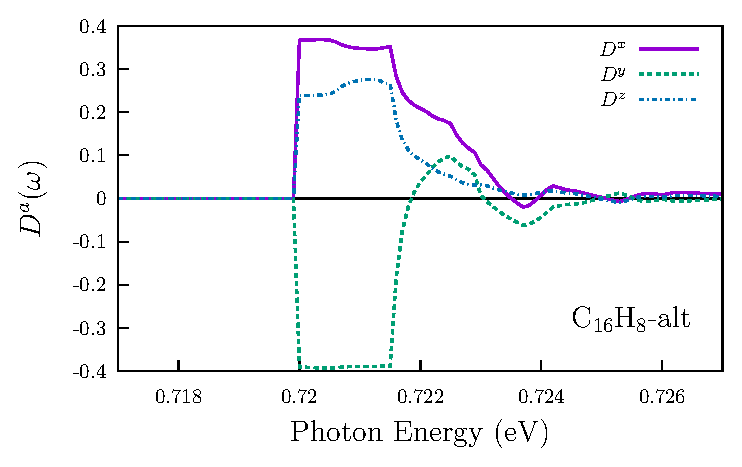
\includegraphics[width=\linewidth]{figures/alt_Da.eps}}
\hfill
\subfloat{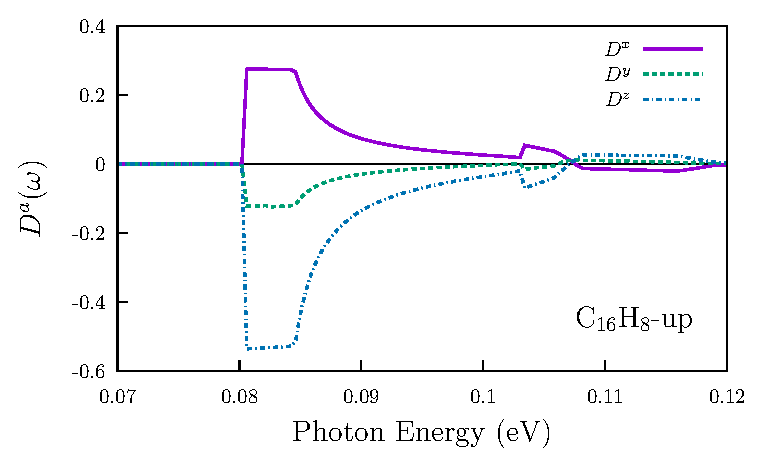
\includegraphics[width=\linewidth]{figures/up_Da.eps}}
\caption{(Color online) Spectra of the degree of spin polarization along the
\emph{a} direction, {$D^{a}(\omega)$}, for the C$_{16}$H$_{8}$-alt and
C$_{16}$H$_{8}$-up structures under incidence of circularly polarized light.\label{fig:Da}}
\end{figure}


\subsection{Optical current injection}\label{subsec:results-eta}

Figs. \ref{fig:alt-eta} and \ref{fig:up-eta} depict the spectra obtained for the current injection tensor components, $\eta^{abc}(\omega)$, from the \emph{alt} and \emph{up} systems. In both figures the solid lines show to the total response of a given component and the dashed lines correspond to the layer by layer response, of hydrogen or carbon, that contributes to that total response. The \emph{alt} system has three layers divided as shown in Table \ref{tab:altstrc}. The first one corresponds to the top hydrogens atoms, the second to the center layer of carbons and the last to the down hydrogen atoms as that can be observed at the right side of Fig. \ref{fig:altstrc}. The \emph{up} system has only two layers divided as shown in Table \ref{tab:upstrc}, the top conformed by hydrogen atoms and the bottom conformed by carbon atoms. From Figs. \ref{fig:alt-eta} and \ref{fig:up-eta} it is possible to see that the $\eta^{xxy}$ and $\eta^{xxy}$ components have contributions from all three layers while the $\eta^{zxy}$ has only contributions from the carbon layer.
\begin{figure}[t]
  \centering
  \subfloat{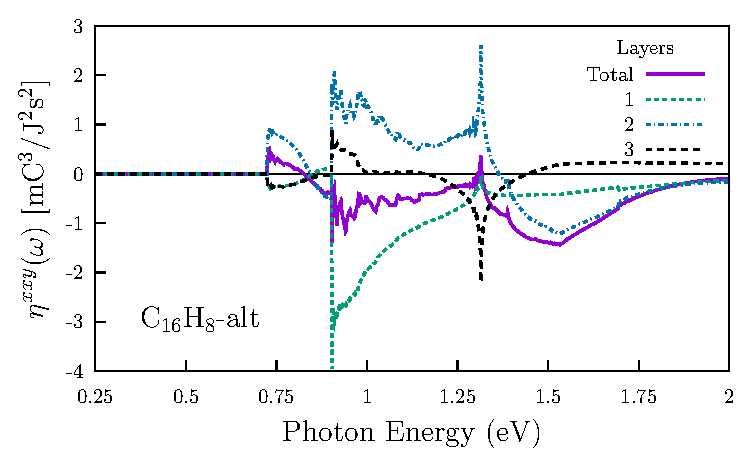
\includegraphics[width=\linewidth]{figures/alt_eta_x.eps}}\\
  \subfloat{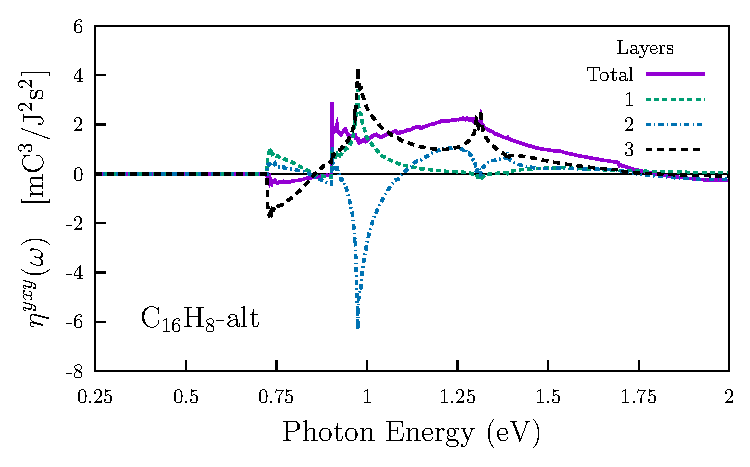
\includegraphics[width=\linewidth]{figures/alt_eta_y.eps}}\\
  \subfloat{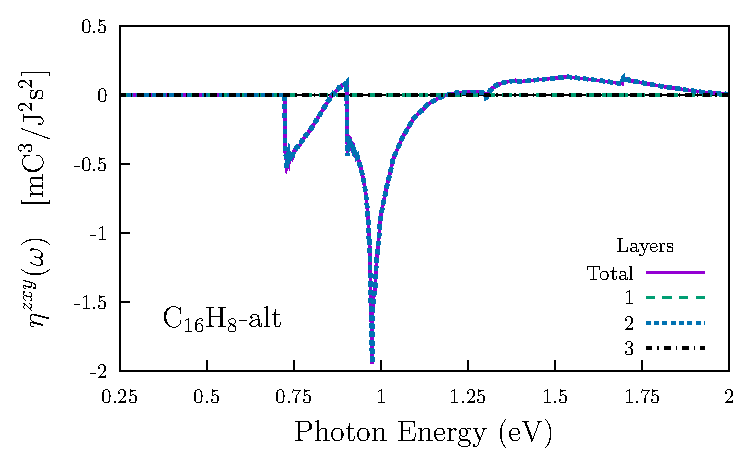
\includegraphics[width=\linewidth]{figures/alt_eta_z.eps}}
  % 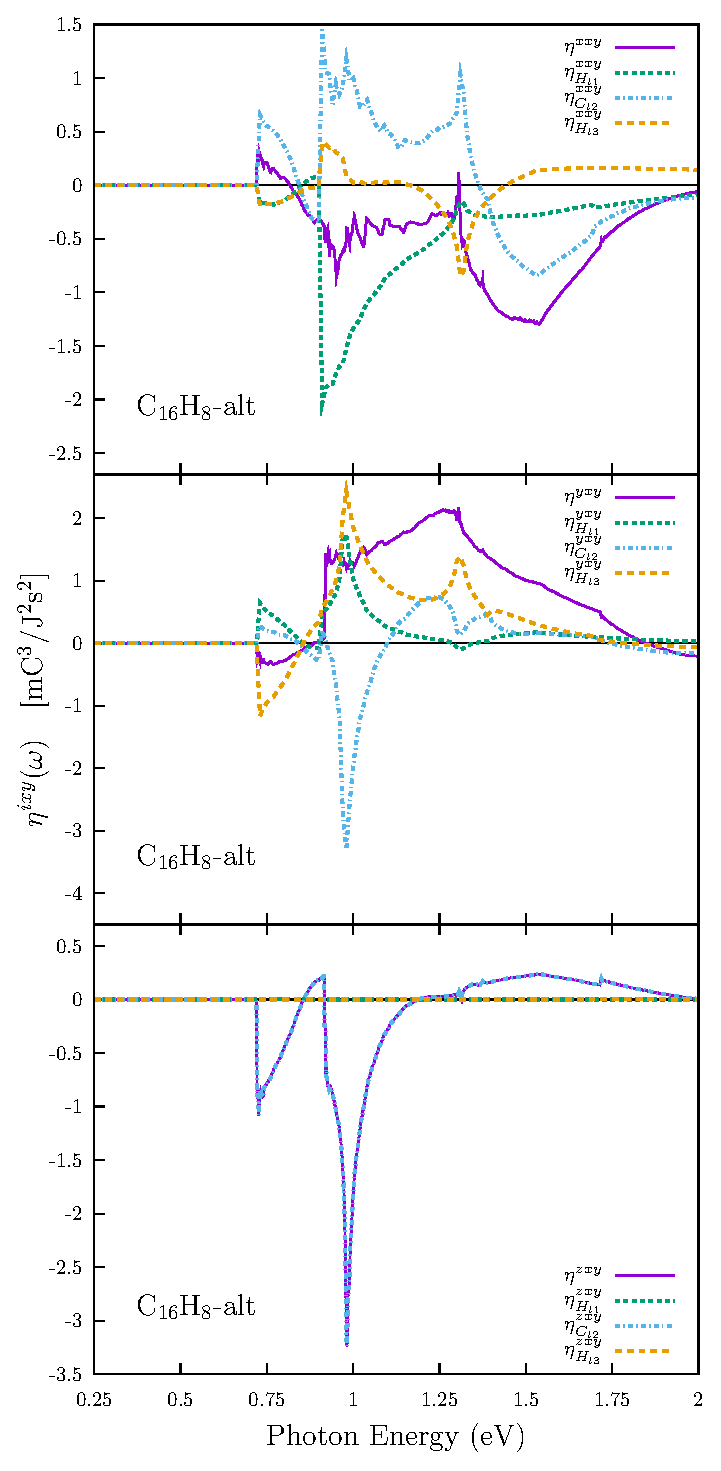
\includegraphics[width=\linewidth]{alt/alt-eta-layers.eps}
  \caption{(Color online) Spectra of the injection current tensor along the \emph{a} direction, {$\eta^{abc}(\omega)$}, layer by layer, for the hydrogenated graphene structure C$_{16}$H$_{8}$-alt under incidence of circularly polarized light.\label{fig:alt-eta}}
\end{figure}

\begin{figure}[b]
  \centering
  \subfloat{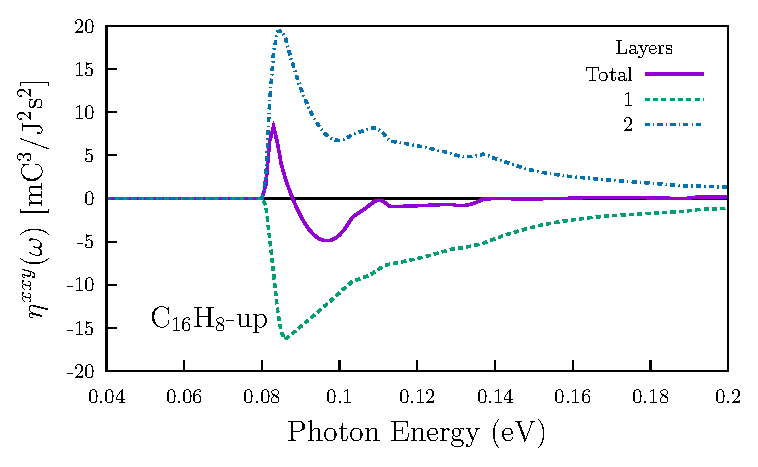
\includegraphics[width=\linewidth]{figures/up_eta_x.eps}}\\
  \subfloat{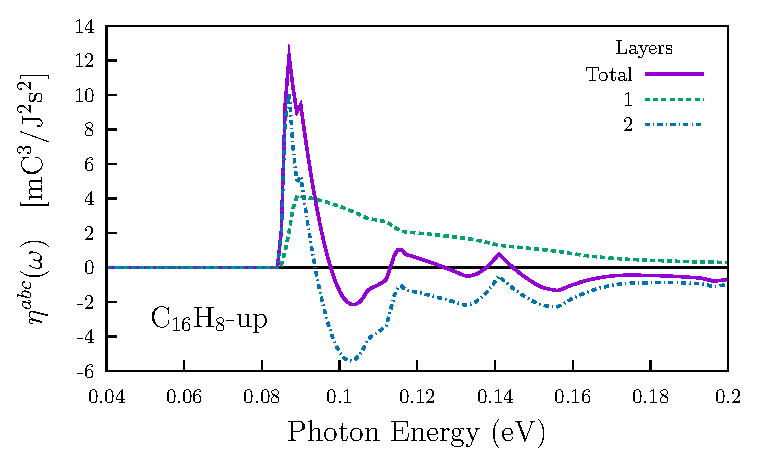
\includegraphics[width=\linewidth]{figures/up_eta_y.eps}}\\
  \subfloat{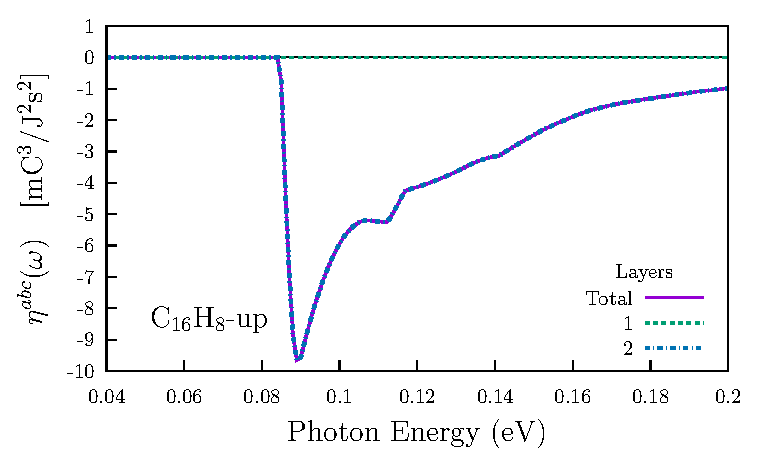
\includegraphics[width=\linewidth]{figures/up_eta_z.eps}}
  % 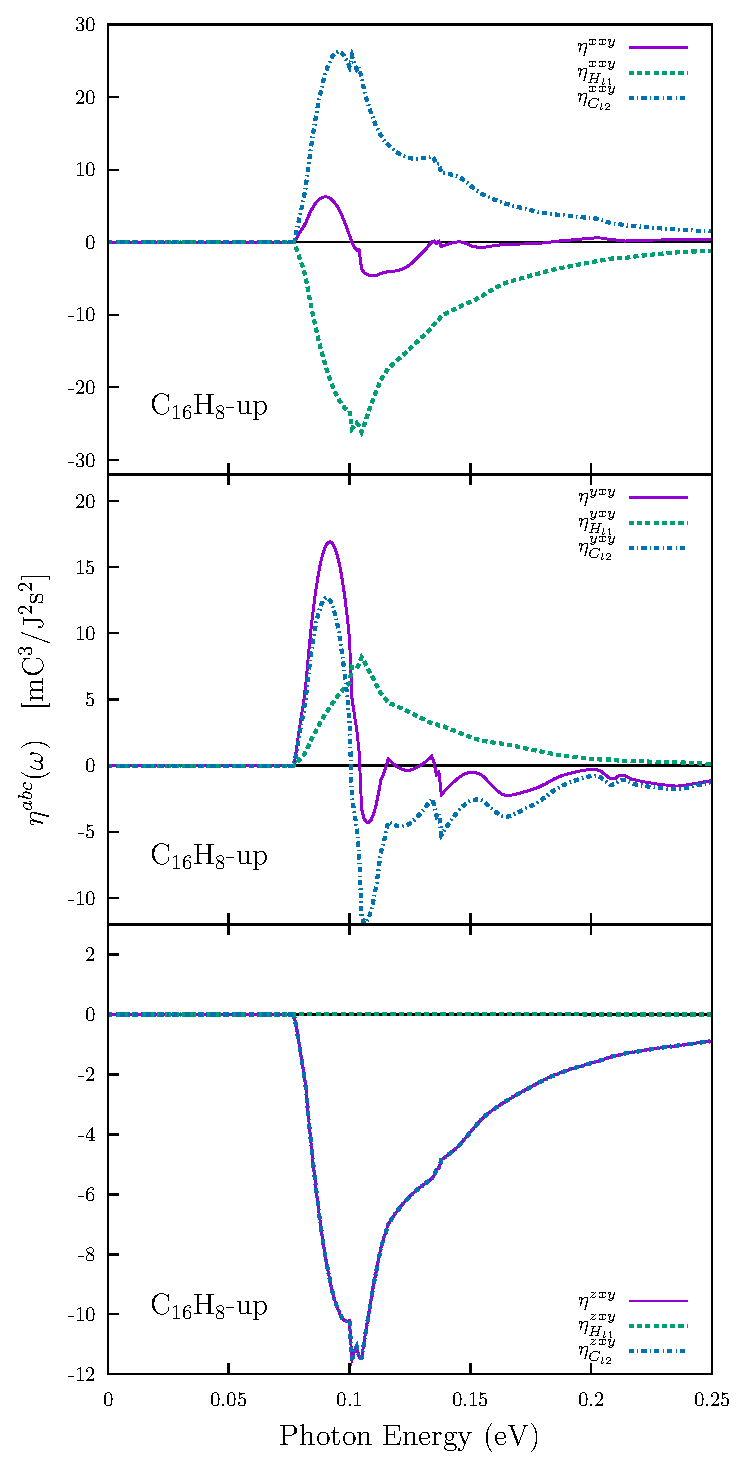
\includegraphics[width=\linewidth]{up/up-eta-multiplot.eps}
  \caption{(Color online) Spectra of the injection current tensor along the \emph{a} direction, {$\eta^{abc}(\omega)$}, layer by layer, for the hydrogenated graphene structure C$_{16}$H$_{8}$-up under incidence of circularly polarized light.\label{fig:up-eta}}
\end{figure}
For the \emph{alt} structure we analyze two important energy values of interest for the response. The first one corresponds for an energy of 0.9\,eV. For this energy the system have important contributions in the all three components. From the figure \ref{fig:alt-eta} we can see that the contributions for the component $\eta^{xxy}(\omega)$ comes for the all three layers having a principal contribution from the first hydrogen layer and reaching a value of $\eta^{xxy}(\omega)$=-0.50\,mC$^{3}$/J$^{2}$s$^{2}$. The $\eta^{yxy}$ component presents contributions again from the all three layers but principally by the carbon and bottom hydrogen layers reaching a value of $\eta^{yxy}$=1.0\,mC$^{3}$/J$^{2}$s$^{2}$. Finally, the $\eta^{zxy}$ component, as mentioned before, has only contributions from the carbon layer reaching a value of -1.9\,mC$^{3}$/J$^{2}$s$^{2}$; the hydrogen layers contributions are identically to zero. Using the Eq. \eqref{eq:etatotal} we have that for this fixed value of energy the total contribution is $\eta^(\omega)$=2.2\,mC$^{3}$/J$^{2}$s$^{2}$ and it is fixed at $\varphi=116^{\circ}$ and $\theta=-135^{\circ}$. The second value of energy of interest is for 1.30\,eV of energy where the absolute maximum of total layers contributions of the spectra is reached with a value of 2.30\,mC$^{3}$/J$^{2}$s$^{2}$ for the $\eta^{yxy}$ component. For this energy the $\eta^{xxy}$=0.5\,mC$^{3}$/J$^{2}$s$^{2}$ and $\eta^{zxy}$ is identical to zero. Also we can see that the contributions for the $\eta^{yxy}$ component come from the carbon and bottom hydrogen layers and that the contributions from the carbon and bottom hydrogen layer for $\eta^{xxy}$ are almost annihilated between themselves. This value is fixed only in the $xy$ plane with $\varphi=78^{\circ}$. In Fig. \ref{fig:altstrc} the green dashed lines depicts only the angles where this two values of $\eta^{zxy}(\omega)$ points for this two energy values energy; they are denoted by $\eta_{1}$ for 0.9\,eV and $\eta_{2}$ for 1.30\,eV. Finally for the \emph{alt} structure  we have that for all the three components the response goes to zero after 1.75\,eV. 

In a similar way than in the previous structure analysis the total value for each component of $\eta^{abc}$ comes from contributions from both layers unless for the  $\eta^{zxy}$ which contributions comes only from the carbon layer. For the \emph{up} case we analyze again two energies of interest, the first for 0.09\,eV and the second for 1.1\,eV. For the first value of energy we have contributions from all the three components. The maximum value of $\eta^{xxy}$=9.0\,mC$^{3}$/J$^{2}$s$^{2}$ is reached for this energy and the contributions for each of the two layers are in opposite directions predominating the contributions from the hydrogen layer. Also the component $\eta^{yxy}$=13\,mC$^{3}$/J$^{2}$s$^{2}$ reaches the absolute maximum of the total response, due to the sum of contributions from both layers. The last component for this energy value is $\eta^{zxy}$=-11\,mC$^{3}$/J$^{2}$s$^{2}$ and as mentioned before, has only contributions from the carbon layer. Using the Eq. \ref{eq:etatotal} we have that the total response for this given value of energy is $\eta(\omega)$=19.3\,mC$^{3}$/J$^{2}$s$^{2}$ fixed at $\varphi=55^{\circ}$ $\theta=-51^{\circ}$. For the second energy value, 1.1\,eV, we have that the $\eta^{xxy}$ and $\eta^{yxy}$ are inverted in direction with respect to the previous energy value reaching values of -4.0\,mC$^{3}$/J$^{2}$s$^{2}$ and -2.5\,mC$^{3}$/J$^{2}$s$^{2}$, respectively. Also, for this energy we have the  contribution of the last component is $\eta^{zxy}$=-5.5\,mC$^{3}$/J$^{2}$s$^{2}$. Using again the Eq. \eqref{eq:etatotal} we have a total response is $\eta^(\omega)$=7.2\,mC$^{3}$/J$^{2}$s$^{2}$ and it is directed in $\varphi=-147^{\circ}$ and $\theta=-126^{\circ}$  angles. In figure \ref{fig:upstrc} the green dashed arrows depicts only the angles where the two $\eta(\omega)$ values point denoted by $\eta_{1}$ for 0.9\,eV and $\eta_{2}$ for 1.1\,eV. Finally we have that for the \emph{up} system the response goes to zero after 0.2\,eV. 

In table \ref{tab:etacomp} we present a comparison of the absolute maximum values of $\eta^{abc}(\omega)$ in a given direction reported for different materials and the corresponding energy at which the maximum value of $\eta^{abc}(\omega)$ is reached. From the table we can see that, excluding the case of the bulk CdSe, the \emph{alt} structure reaches a larger value for $\eta^{abc}(\omega)$ than some of the systems and is in the same order of magnitude that the Si(111) 2$\times$1 system and almost for the same photon energy, 1.25\,eV, which is in the near infrared range. Also, the other layered structures have reported two orders of magnitude lower values for this response. 

The reference \cite{lamanAPL99} includes the results of a one-photon experiments for the optical current injection performed on bulk CdSe. They measured an injection current density of 2\,$\mu$A/cm$^{2}$ that entered 1.8\,$\mu$m deep. In Table \ref{tab:etacomp} we also show the corresponding experimental value for the surface injection current tensor of bulk CdSe.


\begin{table}%
  \sidecaption
  \begin{tabular}{lcccc}
  \hline
    Structure & Energy &  \multicolumn{2}{c}{$\eta^{abc}(\omega)$} &  Ref.\\
    \cline{3-4}
              & [eV]   & $abc$ & [mC$^{3}$/J$^{2}$s$^{2}$] \\
    \hline
    C$_{16}$H$_{8}$-alt     & 1.25  & yxy & 2.30  & *     \\
    C$_{16}$H$_{8}$-up      & 0.09  & yxy & 13.0  & *     \\
    Si(111)-In $8\times2$   & 1.24  & yxy & 0.35  & \cite{arzatePRB14}  \\
    Si(111) $2\times1$      & 0.75  & yxy & 1.22  & \cite{mendozaPRB12} \\
    GaAs(110) clean         & 4.30  & yxy & 0.30  & \cite{nastosPRB07}     \\
    GaS (110)-Sb            & 4.60  & yxy & 0.17  & \cite{cabellosPRB11}\\
    Bulk CdSe               & 1.80  & yyz & 90.0$^{\star}$  & \cite{lamanAPL99}  \\
  \hline
  \end{tabular}
  \caption[]{%
  Comparison of the highest reported absolute values of {$\eta^{abc}(\omega)$} for 
    different structures. ($^{*}$This work. $^{\star}$Experimental value.)}
  \label{tab:etacomp}
\end{table}

\subsection{Second-harmonic generation}
In Figs. \ref{fig:alt-shg-abs} and \ref{fig:up-shg-abs} we show the absolute value of the different nonzero components of $\chi^{abc}$ for both cases resulting from the evaluation of Eqs. \eqref{eq:chis} and \eqref{eq:chitotal}. For the \emph{alt} system, we note that all components except $xxy$ present two peaks at $\sim0.5$\,eV and $\sim1.0$\,eV. The first peak is completely produced by $2\omega$ resonances, while the second peak is produced by a mixture of both $1\omega$ and $2\omega$ resonances, with the latter dominating in most cases. The $xxy$ component has a single broadened peak with a discernible feature near 0.5\,eV. That feature, much like the other components, is produced by $2\omega$ resonances, while the maxima is produced by a mixture of both frequencies, $1\omega$ and $2\omega$. For the \emph{up} structure we see one predominant peak around 0.05\,eV; it is completely produced by $2\omega$ transitions. The $xxy$ and $yxx$ components have an additional feature close to 0.09\,eV dominated by $1\omega$ transitions. In table \ref{tab:shgcomp} we show a comparison of the maximum $\chi^{abc}$ peak reported for different structures.

\begin{figure}[t]
\subfloat{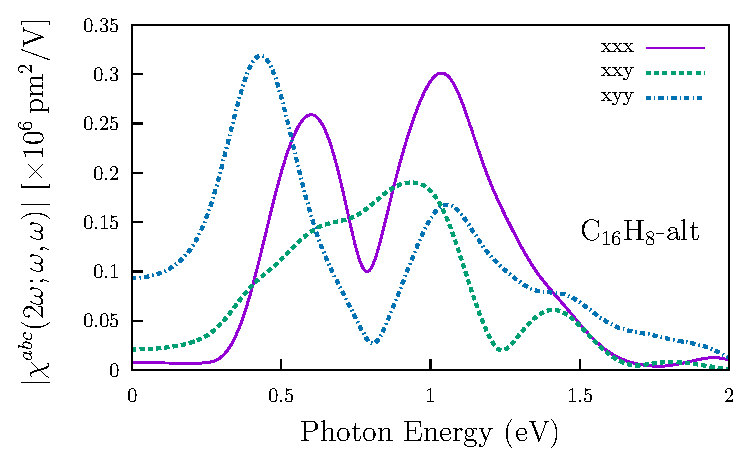
\includegraphics[width=\linewidth]{figures/alt_shg_abs_x.eps}}\\
\subfloat{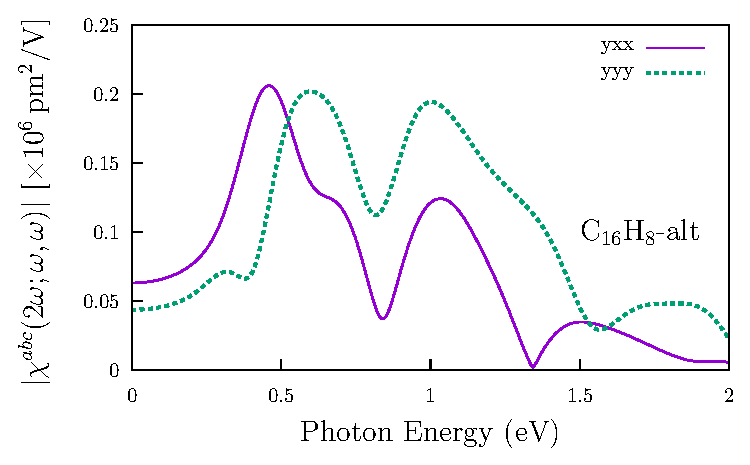
\includegraphics[width=\linewidth]{figures/alt_shg_abs_y.eps}}
\caption{(Color online) Spectra of the absolute value of SHG for the
    C$_{16}$H$_{8}$-alt structure corresponding to the
    sum of the absolute value for the non zero real and imaginary components
    of $\chi^{abc}(2\omega;\omega,
    \omega) $ tensor.\label{fig:alt-shg-abs}}
\end{figure}

\begin{figure}[t]
\subfloat{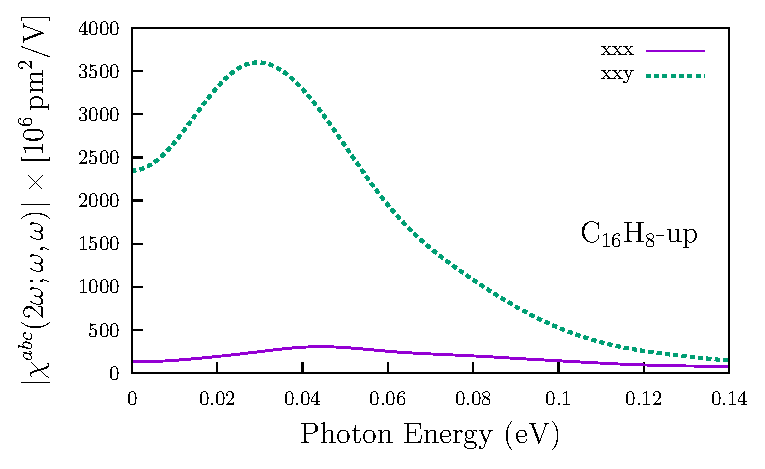
\includegraphics[width=\linewidth]{figures/up_shg_abs_x.eps}}\\
\subfloat{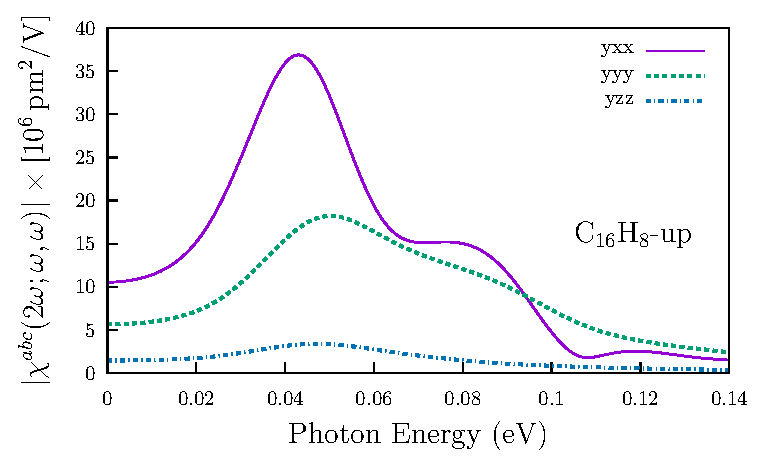
\includegraphics[width=\linewidth]{figures/up_shg_abs_y.eps}}
\caption{(Color online) Spectra of the absolute value of SHG for the
    C$_{16}$H$_{8}$-up structure corresponding to the
    sum of the absolute value for the non zero real and imaginary components
    of $\chi^{abc}(2\omega;\omega,
    \omega) $ tensor.\label{fig:up-shg-abs}}
\end{figure}


\begin{table}[htb]%
  \sidecaption
  \begin{tabular}{lcccc}
  \hline
    Structure & \hspace{-5mm}Energy & \multicolumn{2}{c}{$\chi^{abc} $} &  Ref.\\
    \cline{3-4}
              & \hspace{-5mm}[eV]   & $abc$ & value \\
    \hline
    C$_{16}$H$_{8}$-alt   & \hspace{-5mm}0.4   & xyy   & 0.32\scriptsize{$\times 10^{6}\,\mathrm{pm}^{2}/\mathrm{V}$}  & *     \\
    C$_{16}$H$_{8}$-up    & \hspace{-5mm}0.042 & yxx   & 37  \scriptsize{$\times 10^{6}\,\mathrm{pm}^{2}/\mathrm{V}$}  & *     \\
    Si(100)2$\times$1     & \hspace{-5mm}1.5   & xxx   & 1.5 \scriptsize{$\times 10^{6}\,\mathrm{pm}^{2}/\mathrm{V}$}  & \cite{andersonPRB15}  \\
    BNNT(6,0) pristine    & \hspace{-5mm}5.0   & zzz   & 35\,\scriptsize{pm/V}  & \cite{salazarPRB14} \\
    BNNT(6,0)+4(H$_{2}$)  & \hspace{-5mm}5.0   & zzz   & 33\,\scriptsize{pm/V}  & \cite{salazarPRB14} \\
    BNNT(6,0)+12(H$_{2}$) & \hspace{-5mm}4.8   & zzz   & 15\,\scriptsize{pm/V}  & \cite{salazarPRB14} \\
  \hline
  \end{tabular}
  \caption[]{%
  Comparison of the highest reported absolute values of SHG for 
    different structures and components. ($^{*}$This work.)}
  \label{tab:shgcomp}
\end{table}

\section{Conclusions}\label{sec:conclusions}

We have performed \emph{ab initio} calculations for the optical spin injection (DSP), optical current injection (OCI), and second-harmonic generation (SHG) on the hydrogenated graphene C$_{16}$H$_{8}$-alt and C$_{16}$H$_{8}$-up structures, (Fig. \ref{fig:structures}) using the independent particle approximation (IPA) and the plane wabe basis. Our calculations abour DSP predicts that it is possible to inject spin-polarized electrons along the three cartesian directions, obtaining maxima DSP of the injected electrons of about 39\% and 57\% in the $y$ and $z$ directions  (Fig. \ref{fig:Da}) at the photon energies of around 0.719 and 0.08\,Ha  for the \emph{alt} and \emph{up} cases, respectively. Also there is a range of energy in which this DSP can be held,{\changed from 0.08 to 0.084\,eV and from 0.08 to 0.084\,eV for the \emph{alt} and \emph{up} cases, respectively}. This results predicts that particularly \emph{up} is usable for spintronics proposes because its energy is readily obtainable using terahertz radiation.

Our results about OCI with circularly polarized light (CPL) show that the \emph{alt}  and \emph{up} systems have a response near to 2.30\,mC$^{3}$/J$^{2}$s$^{2}$ and 18.0\,mC$^{3}$/J$^{2}$s$^{2}$ both in the $y$ direction (Figs. \ref{fig:alt-eta}-\ref{fig:up-eta}) for incident beams with energies of around 1.25 and 0.09\,eV. According to measurements done on bulk materials, it is actually possible to measure such amount of OCI. According to this result we can affir that it is possible to control the motion of electrons in both systems but specially in the \emph{up} one in the $y$ direction.

Finally we found that the \emph{alt} and \emph{up} structures present a absolute maximum of 0.32\,$\times10^{6} $\,pm$^{2}$/V and 37.0\,$\times10^{6} $\,pm$^{2}$/V at the photon energies of around 0.40\,eV and 0.042\,eV (Figs. \ref{fig:alt-shg-abs} and \ref{fig:up-shg-abs}). For \emph{alt} and \emph{up} we have that their maximua come from contributions of the 2$\omega$ resonances. From this we comclude that specially with the \emph{up} system is usable to SHG.


\section{Acknowledgment} % (fold)

This work has been supported by \emph{Consejo Nacional de Ciencia y
Tecnolog\'ia} (CONACyT), M\'exico, Grant No. 153930.


\bibliographystyle{pss}
\bibliography{graphane_structures}

\end{document}
